\documentclass[10pt,conference]{IEEEtran}
% SEAMS 2027 research track: 10 pages of content + 2 pages of references, double anonymous.
\usepackage{graphicx}
\usepackage{booktabs}
\usepackage{amsmath}
\usepackage{xcolor}
\usepackage{url}
\usepackage[hidelinks]{hyperref}
\usepackage{cite}

\newcommand{\todo}[1]{\textcolor{red}{[TODO: #1]}}
\newcommand{\RQ}[1]{\textbf{RQ#1}}

\begin{document}

\title{Governed Agent Societies: Runtime Governance and Trace-Based Assurance for LLM-Driven Multi-Agent Self-Adaptive Systems}
\author{\IEEEauthorblockN{Anonymous Authors}\IEEEauthorblockA{Anonymous Affiliations}}
\maketitle

\begin{abstract}
\todo{Rewrite once the LLM results exist. Keep to 150--200 words: problem, framework, testbed, the two or three headline numbers, artifact.}
Agentic systems built from several LLM-driven roles act through tools, share memory, and take actions with real consequences, yet they are mostly described as prompt pipelines and evaluated on final outputs. We model such systems as governed agent societies: multi-role decision processes in which a runtime guard sits inside the transition function, evidence is a first-class object that actions must cite, and every proposal produces a typed trace record. The guard maps onto the analyze and plan steps of a MAPE-K loop with a human on the loop. We instantiate the model in a smart-city operations testbed with eight service roles, four incident families, planted false reports, and approvals that take time and can be refused, and we evaluate LLM-driven roles under five governance modes, from a single agent with the rules in its prompt to roles with rules both in prompts and enforced at runtime. \todo{headline numbers}. Trace metrics expose what final success hides: episodes that succeed while broadcasting unverified or untrue alerts, actions taken without required approval, and evidence cited that does not exist. A trust-adaptive governor quantifies the trade-off between human approval load and the harm of acting where rules are silent. The testbed, traces and scripts are available as an artifact.
\end{abstract}

\begin{IEEEkeywords}
agentic AI, multi-agent systems, self-adaptive systems, runtime governance, runtime assurance, human on the loop, LLM agents, trace-based evaluation
\end{IEEEkeywords}

%=====================================================================
\section{Introduction}
\label{sec:intro}
\todo{Open with one concrete failure taken from a trace: a communication role broadcasting a city-wide alert on a social-media report that a field crew later refutes. Then the general point in two sentences.}

Recent agentic systems use large language models to plan, retrieve evidence, invoke tools, update memory, and coordinate specialised roles over extended horizons~\cite{yao2023react,wu2023autogen,li2023camel}. Many of them are implemented as prompt pipelines or orchestration graphs, yet their behaviour unfolds as sequential, multi-role execution under partial information and operational constraints. A system may reach an acceptable final outcome while following a weak or unsafe trajectory: a tool call may rest on unsupported evidence, a memory update may preserve an unverified claim, a public-facing action may occur without required approval. These are failures of governed execution, not only of output quality, and final-output evaluation does not see them~\cite{cemri2025mast}.

\todo{Why this is a self-adaptive systems problem: the society adapts its workflow at runtime (verification requests, escalation, sanitisation, fallbacks), under uncertainty in evidence and in human availability; the guard is a runtime assurance mechanism; verifier, governor and overseer are analyze and plan; the trace is the knowledge base.}

\todo{Prompted vs enforced governance: putting rules into prompts is what practitioners do today; enforcing them at runtime is what AgentSpec-style work does for single agents~\cite{wang2026agentspec}. Nobody has measured the difference for multi-role societies with human escalation, nor what it costs in human attention.}

This paper makes four contributions.
\begin{enumerate}
    \item A model of \emph{governed agent societies}: roles as policies over structured state, evidence and memory, with the guard inside the transition function, and a mapping of its parts onto MAPE-K (Section~\ref{sec:model}).
    \item A trace schema and a set of assurance metrics for governed execution: attempted and executed violations, trace support coverage, escalation precision and recall, overseer load, silent violation rate, hallucinated evidence, hidden harm (Section~\ref{sec:design}).
    \item An evaluation with LLM-driven roles in a smart-city operations testbed, comparing prompted and enforced governance across models, rule sets and overseer availability, with paired statistics (Section~\ref{sec:results}).
    \item An open testbed, trace dataset and reproduction scripts (Section~\ref{sec:artifact}).
\end{enumerate}

We ask: \RQ{1} Does runtime enforcement reduce executed violations and missed approvals beyond rules placed in prompts, for LLM-driven roles? \RQ{2} What does governance cost in task success, steps, tokens and overseer load? \RQ{3} Which failures does final success hide, and which trace metrics expose them? \RQ{4} Do the effects hold across models, evidence quality, overseer availability and rule strictness? \RQ{5} \todo{only if the second domain happens} Does the framework transfer to a software operations domain without changing guard, traces or metrics?

%=====================================================================
\section{Background and Related Work}
\label{sec:related}

\paragraph{Self-adaptive systems and MAPE-K}
\todo{Kephart and Chess~\cite{kephart2003autonomic}; Salehie and Tahvildari~\cite{salehie2009}; Weyns~\cite{weyns2020}; assurance for self-adaptive systems~\cite{calinescu2018entrust}; LLMs in self-adaptive systems~\cite{li2024llmsas,maper2026}; human on the loop~\cite{li2020explanations}. Two or three sentences each on how the guard, roles and traces map onto these.}

\paragraph{Runtime assurance and enforcement}
\todo{Simplex architecture~\cite{sha2001simplex}; shields for RL~\cite{alshiekh2018safe} and for multi-agent RL~\cite{elsayedaly2021shielding,compositional2025shielding}; runtime enforcement monitors~\cite{falcone2011enforcement}. The guard is in this family; what is new is evidence and provenance as part of the enforced property, human escalation as an outcome, and the trace as the evaluation object.}

\paragraph{Guardrails for LLM agents}
AgentSpec~\cite{wang2026agentspec} defines a rule language and enforces it at runtime for a single LLM agent; GuardAgent~\cite{xiang2025guardagent} and Progent~\cite{shi2025progent} check or constrain tool calls. \todo{Differences: several roles with different visibility, memory notes as evidence, approvals with latency and denial, metrics on traces rather than blocked/allowed counts.}

\paragraph{Evaluating agents on traces}
$\tau$-bench~\cite{yao2025taubench} scores tool agents on compliance with domain policies; the MAST taxonomy~\cite{cemri2025mast} classifies failures of multi-agent LLM systems from their traces. \todo{We turn trace inspection into metrics and compare governance mechanisms with them.}

\paragraph{Normative multi-agent systems}
\todo{Two sentences: electronic institutions and organisational models~\cite{esteva2001ei,hubner2007moise} regulate agent societies by norms and roles; our guard is a lightweight runtime instance of that idea for LLM-driven roles, with evidence and human oversight built in.}

Agentic architectures and memory~\cite{yao2023react,wu2023autogen,li2023camel,park2023generative,packer2023memgpt,shinn2023reflexion} \todo{one paragraph, shortened from the ESEM version.}

%=====================================================================
\section{Governed Agent Societies}
\label{sec:model}

\paragraph{Process model}
An agentic workflow is a \emph{Governed Agent Society Process}
\[
\mathcal{G} = (\mathcal{I}, \mathcal{S}, \{\mathcal{O}_i\}, \{\mathcal{A}_i\}, \mathcal{E}, \mathcal{M}, \mathcal{C}, G, \mathcal{T}, \rho),
\]
with roles $\mathcal{I}$, state space $\mathcal{S}$, role observations $\mathcal{O}_i$ and typed actions $\mathcal{A}_i$, an evidence store $\mathcal{E}$ whose items have an identity, a topic, a status and a visibility, a memory store $\mathcal{M}$ of notes that inherit the status of their source, an active rule set $\mathcal{C}$, a guard $G$, a transition operator $\mathcal{T}$ and an initial distribution $\rho$. \todo{Trim the ESEM text; drop reward $\mathcal{R}$ and discount $\gamma$ from the headline tuple, mention learning as future work in one sentence.}

At step $t$ every active role $i$ observes $o_t^{(i)} = \Omega_i(s_t)$ (its visible evidence, the shared notes, the flags of its service, the guard's answer to its previous proposal, open approval requests) and proposes a typed action $a = \langle r, \alpha, z, p, E, q \rangle$: role, action type, target, payload, cited evidence ids and a self-reported probability $q$ that the action needs approval. The guard maps the proposal to an outcome in \{allow, deny, sanitize, request evidence, escalate\}, and the state moves by $s_{t+1} \sim \mathcal{T}(s_t, \mathbf{a}_t, e_t)$ where $e_t$ carries the guard outcomes and any human answer.

\paragraph{The guard}
Rules run in a fixed order: scope, memory provenance, public communication, evidence, approval, domain-specific sanitisation (Table~\ref{tab:rules}). \todo{Table with the R2 rules, their outcome and the violation label. Say that R1 and R3 are configurations of the same rules.} A proposal is \emph{supported} when it cites at least one verified item on the action's topic, cites nothing refuted, and, for public communication, cites nothing unverified. Approval requests reach the human after a latency, are refused when the request is unsupported or the human is unavailable, and a refusal holds for the episode. The guard reads the risk level of an action from the catalogue, never from the proposal.

\paragraph{One property}
Under the guard, no executed action violates an active rule: violations can only appear as proposals, which the trace records. This is why the paper reports \emph{attempted} and \emph{executed} violations separately, and why executed violations must be exactly zero in every guarded run (a non-zero count is a bug, and the tests assert it).

\paragraph{MAPE-K mapping}
\todo{Figure~\ref{fig:arch} relabelled: Monitor = observations and evidence; Analyze = verifier (support check) and metrics; Plan = governor (rules, escalation) and role policies; Execute = execution interface; Knowledge = evidence store, memory notes, rule set, trace. Human on the loop through the overseer.}

\begin{figure}[t]
\centering
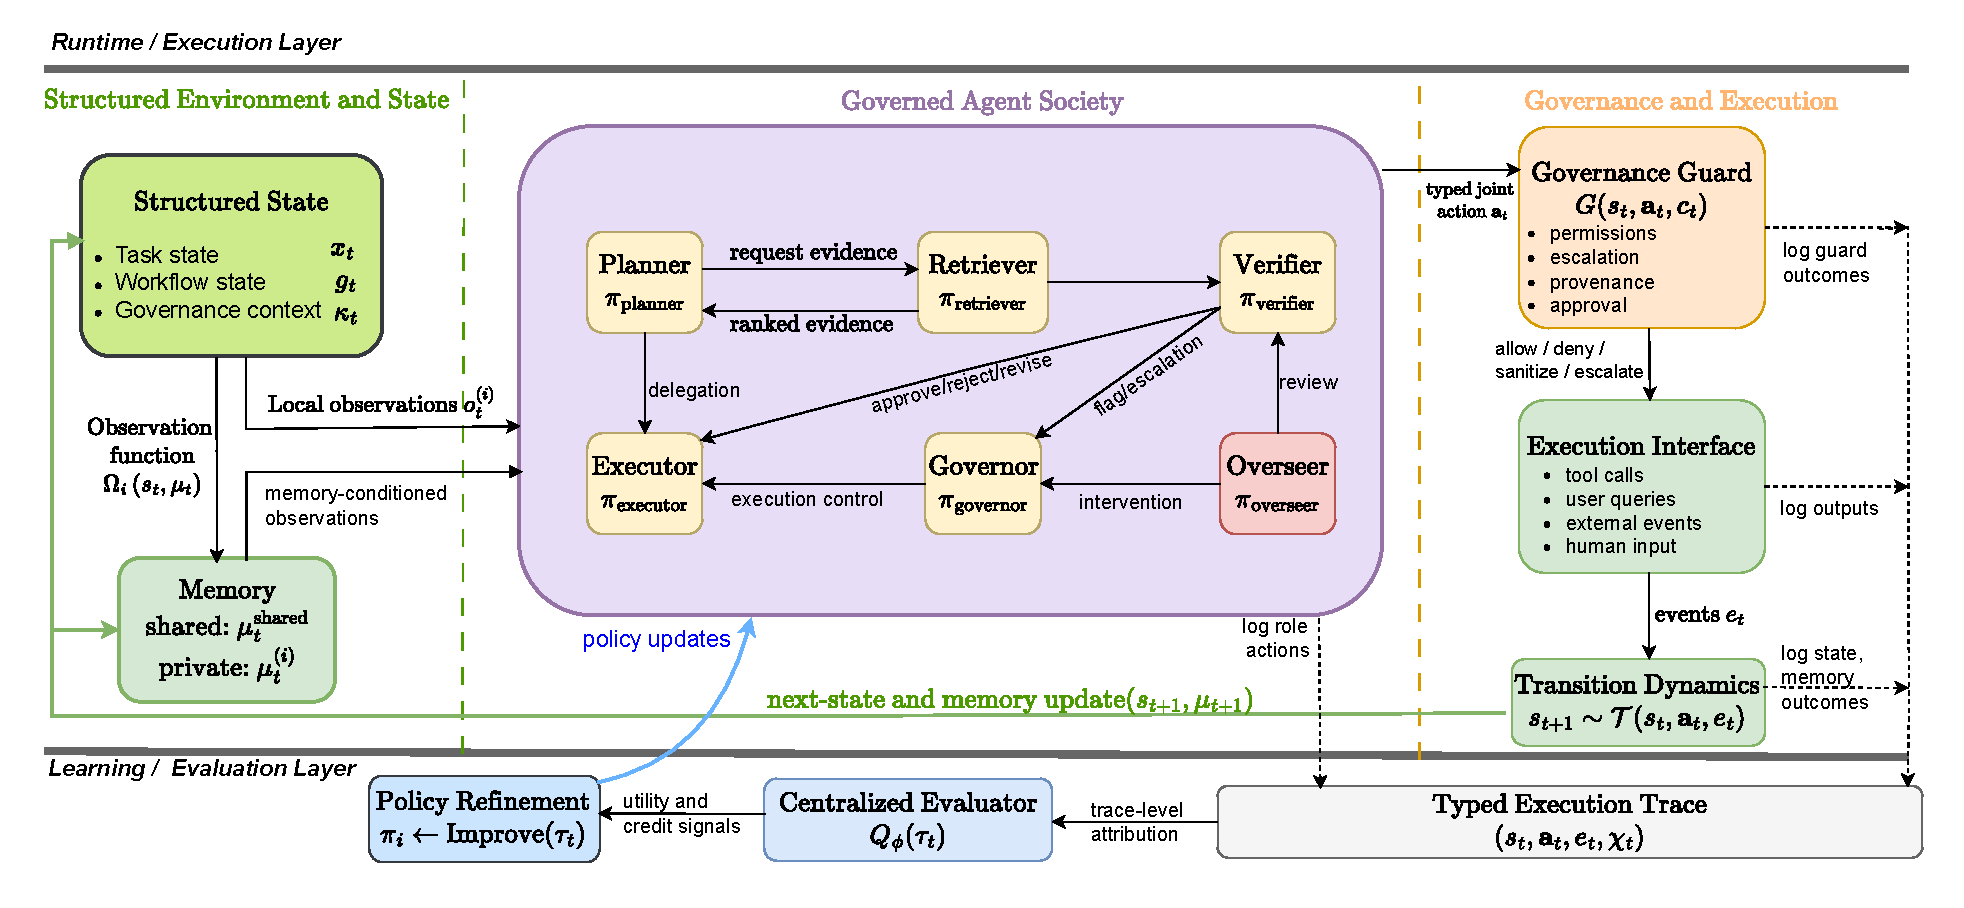
\includegraphics[width=\linewidth]{figures/architecture.pdf}
\caption{Runtime and evaluation architecture. \todo{relabel with MAPE-K terms; move evidence store into the state box.}}
\label{fig:arch}
\end{figure}

\paragraph{Trust-adaptive governor}
\todo{Definition: per-role trust from supported compliant actions (+0.1) and attempted violations (-0.3), carried across incidents; soft approvals delegated when trust is at or above a threshold; hard approvals never. Motivation: earned autonomy in self-adaptive systems; what it costs is measured in Section~\ref{sec:results}.}

%=====================================================================
\section{Testbed}
\label{sec:testbed}

\paragraph{Smart-city operations society}
\todo{Eight service roles and their action catalogues; four incident families with their required roles and success conditions (all need a public alert, so at least three roles must act); one paragraph on why symbolic state.}

\paragraph{Evidence}
\todo{Items E1--E5, F1, D1 with topics, kinds, visibility. Quality levels: complete, partial, missing, conflicting. Verification by topic permission; forwarded requests; memory notes as evidence with inherited status. Planted false report in 25\% of scenarios; distractor in 30\%; hidden context (the overseer would refuse a soft request) in 15\%.}

\paragraph{Scenario generation}
\todo{Stratified 20 per family, seed in the manifest; Table with the feature distributions (from feature\_table.json).}

\paragraph{Role policies}
\todo{LLM roles: prompt structure, the two variants, JSON output, retry, formatting failures. Deterministic references: naive (does not know the rules; adapts only to guard feedback) and procedural (compliant), used as the reachability check and as the lower/upper reference rows.}

%=====================================================================
\section{Evaluation Design}
\label{sec:design}

\paragraph{Modes}
M0 one agent with all tools and the rules in its prompt; M1 roles without rules; M2 roles with rules in prompts only; M3 roles with the guard and no rules in prompts; M4 rules in prompts and the guard. \todo{one sentence on what each pair isolates: M2 vs M3 prompted vs enforced; M0 vs M3 monolith vs society; M3 vs M4 whether knowing the rules reduces the friction of enforcement.}

\paragraph{Metrics}
\todo{Definitions with formulas, from metrics.py's docstring: attempted/executed violations, missed approvals, escalation precision and recall, overseer load and unnecessary share, Brier score of $q$, TSC, hallucinated references, false alert, silent violation rate, hidden harm, GAU with its weights and the weight grid.}

\paragraph{Worked example}
Table~\ref{tab:worked} follows one guarded episode and derives every metric from its trace.
\begin{table*}[t]
\centering
\caption{Worked example: POLL-006 (pollution spike), mode D3-roles-naive-guard}
\label{tab:worked}
\footnotesize
\begin{tabular}{@{}llp{0.22\linewidth}p{0.26\linewidth}lll@{}}
\toprule
\textbf{Step} & \textbf{Role} & \textbf{Action} & \textbf{Evidence} & \textbf{Guard} & \textbf{Rule} & \textbf{Note} \\
\midrule
0 & Pollution & reduce\_traffic\_zone & E1 (verified), E5 (verified) & allow & – &  \\
0 & Traffic & reroute\_traffic & E3 (verified) & sanitize & pollution\_zone & pollution\_zone\_reroute \\
0 & PublicTransport & add\_public\_transport\_capacity & E1 (verified), E3 (verified), E5 (verified) & allow & – &  \\
0 & CitizenComms & broadcast\_alert & E4 (unverified) & request\_evidence & public\_comm & unsupported\_public\_communication \\
1 & Pollution & write\_memory (incident) & E1 (verified) & deny & memory\_provenance & unsupported\_memory\_write \\
1 & CitizenComms & request\_verification (E4) & E4 (unverified) & allow & – &  \\
2 & Pollution & write\_memory (incident) & E1 (verified) & allow & – &  \\
2 & Traffic & request\_verification (E4) & E4 (unverified) & allow & – &  \\
2 & CitizenComms & broadcast\_alert & E4 (verified) & escalate & approval & missed\_approval \\
4 & CitizenComms & broadcast\_alert & E4 (verified) & escalate & approval &  \\
5 & CitizenComms & broadcast\_alert & E4 (verified) & allow & – &  \\
\bottomrule
\end{tabular}

\smallskip
\begin{minipage}{0.96\linewidth}\footnotesize\raggedright
\textbf{Derivation.} proposals (non-noop role actions): 11; environment steps: 6. attempted violations: 4 = pollution\_zone\_reroute $\times$ 1, unsupported\_public\_communication $\times$ 1, unsupported\_memory\_write $\times$ 1, missed\_approval $\times$ 1. executed violations: 0 (executed proposals that broke a rule). missed approvals: 0 (executed actions that required approval and had none). escalations: 1; overseer load (distinct approval requests reaching the human): 1; granted 1, denied 0. escalation precision 1.00, recall 1.00. Brier score of the reported approval probability: 0.36. TSC: executed high-impact actions 3, supported 3 $\rightarrow$ 1.00. hallucinated references: 0 of 16 cited ids $\rightarrow$ 0.00. false alert sent: 0; hidden harm: 0. success: 1; silent violation (success with an executed violation): 0. GAU = success - 0.3$\cdot$executed violations - 0.2$\cdot$missed approvals - 0.1$\cdot$unsupported memory writes - 0.1$\cdot$steps/16 - 0.3$\cdot$hidden harm = 0.96.
\end{minipage}
\end{table*}
 \todo{keep the table from tables/worked\_example.tex, shorten the derivation list to the metrics used in the results.}


\paragraph{Statistics}
The scenario is the unit of analysis; repeats are averaged first. Modes see the same scenarios, so comparisons are paired: Wilcoxon signed-rank tests (no normality assumption; many differences are zero), Cliff's $\delta$ as effect size, 95\% bootstrap confidence intervals (10\,000 resamples) for every mean and mean difference, Holm correction across the metrics of one comparison. \todo{Primary comparisons and hypotheses stated before the results.}

%=====================================================================
\section{Results}
\label{sec:results}

\paragraph{Deterministic reference rows}
Table~\ref{tab:main} \todo{these are the deterministic rows; the LLM table replaces or joins them once the grid has run.}
\begin{table*}[t]
\centering
\caption{Deterministic reference rows, 80 scenarios (20 per family), rule set R2. Naive roles do not know the rules; procedural roles follow them. Att.\ viol.\ = attempted, Exec.\ viol.\ = executed violations per episode; Overseer = approval requests reaching the human per episode; Silent viol.\ = share of successful episodes with an executed violation.}
\label{tab:main}
\footnotesize
\begin{tabular}{lcccccccccccc}
\toprule
\textbf{Mode} & \textbf{Succ.} & \textbf{Steps} & \textbf{Prop.} & \textbf{Att. viol.} & \textbf{Exec. viol.} & \textbf{Miss. appr.} & \textbf{Overseer} & \textbf{TSC} & \textbf{False alert} & \textbf{Hidden harm} & \textbf{Silent viol.} & \textbf{GAU} \\
\midrule
D0 direct naive noguard & 1.00 & 3.95 & 3.95 & 2.00 & 2.00 & 0.06 & 0.00 & 0.20 & 0.33 & 0.07 & 0.99 & 0.34 \\
D0g direct naive guard & 1.00 & 7.88 & 7.61 & 2.39 & 0.00 & 0.00 & 0.64 & 1.00 & 0.00 & 0.00 & 0.00 & 0.95 \\
D1 all naive noguard & 1.00 & 1.25 & 5.08 & 2.96 & 2.96 & 0.06 & 0.00 & 0.16 & 0.24 & 0.07 & 1.00 & 0.07 \\
D1g all naive guard & 1.00 & 4.49 & 12.78 & 5.16 & 0.00 & 0.00 & 0.64 & 1.00 & 0.00 & 0.00 & 0.00 & 0.97 \\
D2 roles naive noguard & 1.00 & 1.25 & 4.19 & 2.08 & 2.08 & 0.06 & 0.00 & 0.16 & 0.24 & 0.07 & 1.00 & 0.33 \\
D3 roles naive guard & 1.00 & 4.49 & 11.53 & 3.91 & 0.00 & 0.00 & 0.64 & 1.00 & 0.00 & 0.00 & 0.00 & 0.97 \\
D4 roles procedural noguard & 1.00 & 4.54 & 9.96 & 0.00 & 0.00 & 0.00 & 0.64 & 1.00 & 0.00 & 0.00 & 0.00 & 0.97 \\
D5 roles procedural guard & 1.00 & 4.54 & 9.96 & 0.00 & 0.00 & 0.00 & 0.64 & 1.00 & 0.00 & 0.00 & 0.00 & 0.97 \\
D6 direct procedural noguard & 1.00 & 6.96 & 6.50 & 0.00 & 0.00 & 0.00 & 0.64 & 1.00 & 0.00 & 0.00 & 0.00 & 0.96 \\
D6g direct procedural guard & 1.00 & 6.96 & 6.50 & 0.00 & 0.00 & 0.00 & 0.64 & 1.00 & 0.00 & 0.00 & 0.00 & 0.96 \\
\bottomrule
\end{tabular}

\end{table*}

\paragraph{RQ1 Enforcement vs prompting}
\todo{LLM results M2 vs M3 vs M4 per model; paired stats table.}

\paragraph{RQ2 Cost}
\todo{success, steps, proposals, tokens, overseer load; the R3 and overseer-unavailable rows where success drops.}

\paragraph{RQ3 What success hides}
\todo{silent violation rate, false alerts, unsupported alerts, hallucinated references, hidden harm; the failure catalogue from traces.}

\paragraph{RQ4 Robustness}
\todo{per model, per family, R1/R3, overseer availability sweep; GAU weight grid: how often each mode ranks first.}

\paragraph{Adaptive governor}
Figure~\ref{fig:tradeoff} \todo{describe: under R3 the static guard costs 14\% success when the human is unavailable and puts two requests per incident on the human; delegating soft approvals to trusted roles removes both and exposes the system to every hidden-context case (16\% of episodes). Trust earned by compliance carries no information about what the rules do not encode.}
\begin{figure}[t]
\centering
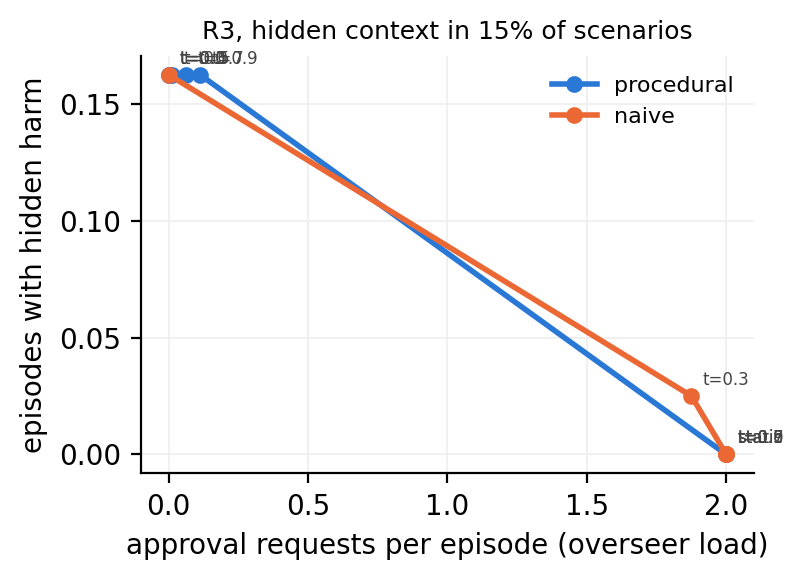
\includegraphics[width=0.9\linewidth]{figures/tradeoff_R3_15.png}
\caption{Overseer load against hidden harm for static and trust-adaptive governance, rule set R3, hidden context in 15\% of scenarios. \todo{redraw for print: one label per distinct point.}}
\label{fig:tradeoff}
\end{figure}

%=====================================================================
\section{Discussion}
\label{sec:discussion}
\todo{How an engineer instantiates the framework: action catalogue with risk and evidence topics, rule set as data, roles with visibility, traces, metrics; what the metrics told us that success did not; the overseer load trade-off; limits of prompted governance.}

\paragraph{Threats to validity}
\todo{Construct: symbolic testbed, rules chosen by us, hidden context modelled as a coin flip. Internal: the naive policy's reactions are ours; LLM nondeterminism handled by repeats. External: one domain (two if RQ5), few models, deterministic overseer. Conclusion: paired tests with Holm, intervals reported, seeds and manifests published.}

%=====================================================================
\section{Conclusion}
\label{sec:conclusion}
\todo{Three sentences.}

\section*{Artifact}
\label{sec:artifact}
\todo{Anonymous link. Testbed, rule sets, prompts, scenario sets, JSONL traces, one-command reproduction, statistics scripts, manifests.}

\bibliographystyle{IEEEtran}
\bibliography{references}

\end{document}
